\documentclass
{article}
\usepackage[margin=1in]{geometry}

\usepackage{authblk}

\title{Constraint Optimization of MicroPlate Designs:\\supplementary materials}
\author{Ramiz Gindullin\textsuperscript{\rm 1}, Mar\'ia~Andre\'ina Francisco~Rodr\'iguez\textsuperscript{\rm 1}}
\affil{\small
    \textsuperscript{\rm 1}Uppsala University, Sweden\\
    {Ramiz.Gindullin@it.uu.se}, {Maria.Andreina.Francisco@it.uu.se}
}


%%%%%%%%%%%%%%%%%%%%%%%%%%%%%%%%%%%%%%%%%%%%%%%%%%%%%%

\usepackage[dvipsnames]{xcolor} % Must be used before tikz and todonotes
\usepackage{todonotes}
\usepackage{tikz}
\usepackage[customcolors,shade]{hf-tikz}
\usetikzlibrary{shapes,arrows,automata,backgrounds,fit,matrix,decorations.pathmorphing,trees,calc,decorations,decorations.text,decorations.markings,decorations.footprints,mindmap,external,arrows.meta,positioning,fadings,shapes.arrows,shadows}
\usepackage{fancyhdr} %Draft date
%\usepackage[nodayofweek]{datetime} %Draft date
%\usepackage[bookmarks=false,hidelinks]{hyperref} %\url used in references 
\usepackage{amsmath}
\usepackage{amssymb} %\nsubseteq
\usepackage{nicefrac}
\usepackage{romannum}
\AtBeginDocument{\pagenumbering{arabic}}
\usepackage{tabularx}
\usepackage{booktabs}
\usepackage{multirow}
\usepackage{multicol}
\usepackage{graphicx} %Include jpg
\usepackage{mathtools}  % provides \coloneqq
\usepackage[inline]{enumitem} %inline lists
\usepackage[T1]{fontenc}  % helps get `<' to show correctly in math mode
\usepackage{titlecaps} %to get title case sentences 
\usepackage[misc]{ifsym} % Envelope symbol for corresponding author
\usepackage{subcaption}

%\usepackage[protrusion=false,expansion=false]{microtype} %needed to
                                %fix ligatures introduced by fontenc
%\usepackage{microtype} %the default options increase the spacing

%\usepackage{orcidlink} % ORCID logo

%\usepackage{subcaption} %subfigures
%\captionsetup[sub]{font=small} %subfigures

\usepackage{textcomp} %\textnumero
\usepackage{verbatim}
\usepackage{soul}
\usepackage{pgfgantt}

%\usepackage{natbib}
%% disable the << and >> ligatures in typewriter type
%\DisableLigatures[<,>]{encoding=T1}

%\usepackage[hidelinks]{hyperref} %already used in line 7
%\urlstyle{same}  %% consider this!!

%%% Mathematics %%%
\newcommand{\setname}[1]{\mathcal{#1}}
\newcommand{\set}[1]{\{#1\}} 


%%% New Colors %%%
\colorlet{LightLavender}{Lavender!50}
\colorlet{LightViolet}{Violet!20}

%%% Todo Notes and Comments %%%
\newcommand{\noteA}[2][]{\todo[#1,color=LightLavender,linecolor=WildStrawberry,bordercolor=WildStrawberry]{#2}\ } %Note by Andreina
\newcommand{\commentA}[2]{\sethlcolor{LightLavender}\hl{#1}\noteA{#2}} %Comment to Andreina
\newcommand{\todoA}[2][]{\todo[#1,color=Violet!20,linecolor=Violet,bordercolor=Violet]{TODO: #2}} %to-do

\newcommand{\todotext}[1]{\textcolor{red}{[#1]}}

\newcommand{\noteR}[2][]{\todo[#1,color=Green!20,linecolor=Green,bordercolor=Green]{#2}\ } %Note to Ramiz
\newcommand{\todoR}[2][]{\todo[#1,color=Green!20,linecolor=Green,bordercolor=Violet]{Question: #2}} %to-do
\newcommand{\commentR}[2]{\sethlcolor{Green!20}\hl{#1}\noteR{#2}} %Comment to Ramiz


%%% Synonyms (used for easy term replacement if needed)
\newcommand{\target}{destination}
\newcommand{\Target}{Destination}


%%% Constraint names %%%
\newcommand{\Constraint}[1]{\textnormal{\textsc{#1}}}
\newcommand{\alldiff}{\Constraint{AllDifferent}}
\newcommand{\Automaton}{\Constraint{Automaton}}
\newcommand{\RegisterAutomaton}{\Constraint{RegisterAutomaton}}
\newcommand{\GenericConstraint}{\Constraint{C}}
\newcommand{\Tcons}{\Constraint{Trans}}
\newcommand{\Tconslong}[5]{\Tcons({#1},{#3},{#5},{#2},{#4})}
\newcommand{\Table}{\Constraint{Table}}
\newcommand{\Regular}{\Constraint{Regular}}
\newcommand{\RegularCounting}{\Constraint{RegCount}}
\newcommand{\RegularCountingAtLeast}{\Constraint{RegCountAtLeast}}
\newcommand{\RegularCountingAtMost}{\Constraint{RegCountAtMost}}
\newcommand{\CostRegular}{\Constraint{CostRegular}}
\newcommand{\MulticostRegular}{\Constraint{MulticostRegular}}
\newcommand{\Lexalldiff}{\Constraint{LexAllDifferent}}
\newcommand{\LexChainGt}{\Constraint{LexChain}}


\newcounter{example}
\newtheorem{example}{Example}


\newcommand{\ECIC}{$\text{IC}_{50}$/$\text{EC}_{50}$}

\begin{document}


\maketitle

\begin{abstract}
    We present detailed results of computational experiments of the paper published in the proceedings of the 2026 AAAI conference~\cite{gindullin26compd}.
\end{abstract}

\section*{Overview}

Here we provide the complete list of figures and tables containing replicated results of replicated experiments~\cite{replicated_experiments} of the paper~\cite{plaid2023} (we will use `the PLAID paper' for brevity):

\begin{itemize}
    \item Figures~\ref{fig:dose_response_paper} and \ref{fig:screening} correspond to Figures~2 and 3 (resp.) of the PLAID paper;

    \item Figures~\ref{fig:dose-response-curves}--\ref{fig:screening-ssmd-collection-10-10-stdev-3} correspond to Figures~1--24 (resp.) from the supplementary materials of the PLAID paper,

    \item Tables~\ref{tab:pvalues-ic50-half-columns-neg-controls-0.4}--\ref{tab:screening-pr_pvalues-10-10-0.2} correspond to Tables~1--5 (resp.) from the supplementary materials of the PLAID paper.
\end{itemize}

Figures~\ref{fig:dose_response_paper}  and Figures~\ref{fig:dose-response-curves}--\ref{fig:dr_percentage_column_neg} showcase various results of dose-response experiments.

Figures~\ref{fig:screening}  and Figures~\ref{fig:screening-data-collection-mild}--\ref{fig:screening-ssmd-collection-10-10-stdev-3} showcase various results of screening experiments.


\begin{figure*}
  \centering
  \begin{subfigure}[c]{\textwidth}
    \centering
    \caption{Examples of dose-response curves with $3$ replicates}
    {\footnotesize Random} \hspace{3.85cm} {\footnotesize PLAID} \hspace{3.45cm} {\footnotesize COMPD}

    
\includegraphics[width=0.3\textwidth]{figures/plate_layout_rand_02.npy_compound_4-right-half.png}
    \label{fig:dr-curves-half-right}
    \hfill
    
\includegraphics[width=0.3\textwidth]{figures/plate_layout_20-12-8-3_01.npy_compound_4-right-half.png}
    \hfill
    
\includegraphics[width=0.3\textwidth]{figures/plate_layout_40-12-8-3_01.npy_compound_4-right-half.png}
    
  \end{subfigure}
  
  \vspace{0.3cm}

  %%%%%%%%%%%

     \begin{subfigure}[b]{0.5\textwidth}
         \centering
         \caption{Residuals}
         
\includegraphics[width=\textwidth]{figures/residuals-1-2-3-8doses-dil8-half-columns-neg-controls-0.4_paper.png}
         \label{fig:residuals-8-doses-half-right}
       \end{subfigure}
       \hfill
       \begin{subfigure}[b]{0.49\textwidth}
         \centering
         \caption{Mean absolute d (max) difference}
         
\includegraphics[width=\textwidth]{figures/dose-response-d_diff-1-2-3-8doses-dil8-right-half-neg-controls-0.4_paper.png}
       \end{subfigure}


  %%%%%%%%%%%

  
     \begin{subfigure}[c]{0.48\textwidth}
         \centering
         \caption{Relative $\text{IC}_{50}$/$\text{EC}_{50}$}
         
\includegraphics[width=\textwidth]{figures/dose-response-relic50-1-2-3-8doses-dil8-half-columns-neg-controls-0.4_paper.png}
         \label{fig:relic50-8-doses-half-right} 
       \end{subfigure}
       %\hfill
       \begin{subfigure}[c]{0.5\textwidth} 
         \centering
         \caption{Absolute $\text{IC}_{50}$/$\text{EC}_{50}$}
         \includegraphics[width=\textwidth]{figures/dose-response-absic50-1-2-3-8doses-dil8-right-half-neg-controls-0.4_paper.png}
         \label{fig:absic50-8-doses-half-right}
     \end{subfigure}

%%%%%
     \caption{Comparison between expected and
       obtained values for dose response curves with
       $8$ doses, $1$, $2$, or $3$ replicates, $20$ negative controls on
       384-well plate, and strong plate effects with a linear relationship to column number on the right side of the plate. %, 
       * indicates ${p<10^{-4}}$, ** indicates ${p<10^{-12}}$, ***
    indicates ${p<10^{-43}}$.}
        \label{fig:dose_response_paper}
\end{figure*}


%%% Local Variables: 
%%% mode: latex
%%% TeX-master: "main.tex"
%%% End: 



\begin{figure*}
  \begin{subfigure}[b]{0.32\textwidth}
    \centering
    \caption{Random}
    
\includegraphics[width=\textwidth]{figures/screening-bowl-0.06-10-10-0.99-stdev-3-4-random.png}
    \label{fig:screen-data-random}
  \end{subfigure}    
  \hfill
  \begin{subfigure}[b]{0.32\textwidth}
    \centering
    \caption{PLAID}
    
\includegraphics[width=\textwidth]{figures/screening-bowl-0.06-10-10-0.99-stdev-3-4-plaid.png}
    \label{fig:screen-data-plaid}
  \end{subfigure}
  \hfill
  \begin{subfigure}[b]{0.32\textwidth}
    \centering
    \caption{COMPD}
    
\includegraphics[width=\textwidth]{figures/screening-bowl-0.06-10-10-0.99-stdev-3-4-compd.png}
    \label{fig:screen-data-compd}
  \end{subfigure}

  
  \begin{subfigure}[b]{0.49\textwidth}
    \centering
    \caption{Z' factor}
    
\includegraphics[width=\textwidth]{figures/screening-Zfactor-mse-manuscript.png}
    \label{fig:zpfactor-mse}
  \end{subfigure}
  \hfill
  \begin{subfigure}[b]{0.47\textwidth}
    \centering
    \caption{SSMD}
    
\includegraphics[width=\textwidth]{figures/screening-SSMD-mse-manuscript.png}
    \label{fig:ssmd-mse}
  \end{subfigure}

  
  \begin{subfigure}[b]{0.49\textwidth}
    \centering
    \caption{1\% hits}
    
\includegraphics[width=\textwidth]{figures/PR-10-10-0.2-1.png}
    \label{fig:screening-pr-10-10-1}
  \end{subfigure}
  \hfill
  \begin{subfigure}[b]{0.49\textwidth}
    \centering
    \caption{5\% hits}
    
\includegraphics[width=\textwidth]{figures/PR-10-10-0.2-5.png}
    \label{fig:screening-pr-10-10-5}
  \end{subfigure}
  
  
  \caption{Screening experiments consisting of 40 microplates for each type of layout, each
    with 10~positive and 10~negative controls and only
    1~replicate per compound. 
    %
    Hits are randomly distributed on each plate.  %
  %
  (a)-(c):~Simulated response data with 1\% hit rate after error correction and normalisation in the presence of mild bowl-shaped plate effects.
  %
    MSE between expected and obtained (d)~Z'~factor and (e)~SSMD in the presence of mild bowl-shaped plate effects. The expected
      values were calculated using plates randomly filled with 50\% positive controls and 50\% negative controls, constituting the optimal values obtainable by these metrics.
  %
  (f) and (g):~PR (precision recall) curves for experiments with
    varying hit rates in the presence of strong bowl-shaped plate
    effects. }
    \label{fig:screening}
\end{figure*}




%%% Local Variables: 
%%% mode: latex
%%% TeX-master: "main.tex"
%%% End: 


\begin{figure*}
  \centering
  \begin{subfigure}[b]{0.05\textwidth}
    ~
  \end{subfigure}
  \hfill
  \begin{subfigure}[b]{0.3\textwidth}
    \centering
    ~~~~~\textbf{Random layout}
  \end{subfigure}
  \hfill 
  \begin{subfigure}[b]{0.3\textwidth}
    \centering
    ~~~~~~\textbf{PLAID layout}
  \end{subfigure}
  \hfill
  \begin{subfigure}[b]{0.3\textwidth}
    \centering
    ~~~~~~\textbf{COMPD layout}
  \end{subfigure}



  \begin{subfigure}[c]{0.05\textwidth}
    
\begin{tikzpicture}
      \node[rotate=90] {~~~~~~~$IC_{50} = 53.43$};  
    \end{tikzpicture}
  \end{subfigure}  
  \hfill
  \begin{subfigure}[c]{0.3\textwidth}
    \centering
    
\includegraphics[width=0.9\textwidth]{figures/plate_layout_rand_02.npy_compound_1-right-half.png}
    \caption{$R^2=0.91$, $IC_{50}=61.92$}
    \label{fig:dr-borer-comp1}
  \end{subfigure}
  \hfill
  \begin{subfigure}[c]{0.3\textwidth}
    \centering
    
\includegraphics[width=0.9\textwidth]{figures/plate_layout_20-12-8-3_01.npy_compound_1-right-half.png}
    \caption{$R^2=0.95$, $IC_{50}=55.48$}
    \label{fig:dr-rand-comp1}
  \end{subfigure}
  \hfill
    \begin{subfigure}[c]{0.3\textwidth}
    \centering
    
\includegraphics[width=0.9\textwidth]{figures/plate_layout_40-12-8-3_01.npy_compound_1-right-half.png}
    \caption{$R^2=0.95$, $IC_{50}=57.66$}
    \label{fig:dr-plaid-comp1}
  \end{subfigure}


  \vspace{5 mm}
  \begin{subfigure}[c]{0.05\textwidth}
    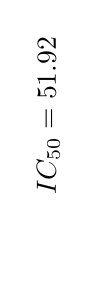
\begin{tikzpicture}
      \node[rotate=90] {~~~~~~~$IC_{50}=51.92$};  
    \end{tikzpicture}
  \end{subfigure}
  \hfill
  \begin{subfigure}[c]{0.3\textwidth}
    \centering
    
\includegraphics[width=0.9\textwidth]{figures/plate_layout_rand_02.npy_compound_4-right-half.png}
    \caption{$R^2=0.95$, $IC_{50}=66.16$}
    \label{fig:dr-border-comp5}
  \end{subfigure} 
  \hfill
  \begin{subfigure}[c]{0.3\textwidth}
    \centering
    
\includegraphics[width=0.9\textwidth]{figures/plate_layout_20-12-8-3_01.npy_compound_4-right-half.png}
    \caption{$R^2=0.96$, $IC_{50}=39.99$}
    \label{fig:dr-random-comp5}
  \end{subfigure}
      \hfill
    \begin{subfigure}[c]{0.3\textwidth}
    \centering
    
\includegraphics[width=0.9\textwidth]{figures/plate_layout_40-12-8-3_01.npy_compound_4-right-half.png}
    \caption{$R^2=0.93$, $IC_{50}=53.02$}
    \label{fig:dr-plaid-comp5}
  \end{subfigure}




  \vspace{5 mm}
  \begin{subfigure}[c]{0.05\textwidth}
    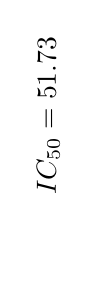
\begin{tikzpicture}
      \node[rotate=90] {~~~~~~~$IC_{50}=51.73$};  
    \end{tikzpicture}
  \end{subfigure}  
  \hfill
  \begin{subfigure}[c]{0.3\textwidth}
    \centering
    
\includegraphics[width=0.9\textwidth]{figures/plate_layout_rand_02.npy_compound_9-right-half.png}
    \caption{$R^2=0.90$, $IC_{50}=17.19$}
    \label{fig:dr-border-comp9}
  \end{subfigure}
  \hfill
  \begin{subfigure}[c]{0.3\textwidth}
    \centering
    
\includegraphics[width=0.9\textwidth]{figures/plate_layout_20-12-8-3_01.npy_compound_9-right-half.png}
    \caption{$R^2=0.91$, $IC_{50}=46.57$}
    \label{fig:dr-random-comp9}
  \end{subfigure}
  \hfill
    \begin{subfigure}[c]{0.3\textwidth}
    \centering
    
\includegraphics[width=0.9\textwidth]{figures/plate_layout_40-12-8-3_01.npy_compound_9-right-half.png}
    \caption{$R^2=0.93$, $IC_{50}=56.59$}
    \label{fig:dr-plaid-comp9}
  \end{subfigure}


  \caption{Examples of dose response curves for simulated experiments
    using 8~doses with 3~replicates (blue dots), 4~negative controls
    (yellow stars), and strong bowl-shaped plate effects. On the left
    of each row we show the expected $IC_{50}$ value. On the caption
    below each plot we show the obtained $R^2$ and $IC_{50}$ values.}
  \label{fig:dose-response-curves} 
\end{figure*}








%%% Local Variables: 
%%% mode: latex
%%% TeX-master: "../supplement.tex"
%%% End: 

\input{tikz-figures/dose_response_d_dist_bowl_no_neg}
\begin{figure*}
  \centering
  \begin{subfigure}[b]{0.05\textwidth}
    ~
  \end{subfigure}
  % 
  \begin{subfigure}[b]{0.45\textwidth}
    \centering
    ~~\textbf{Mild plate effects}
  \end{subfigure}
  % 
  \begin{subfigure}[c]{0.45\textwidth}
    \centering
    ~~\textbf{Strong plate effects}
  \end{subfigure}

  \begin{subfigure}[c]{0.05\textwidth} 
    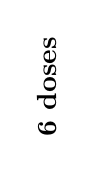
\begin{tikzpicture}
      \node[rotate=90] {\textbf{6 doses}};  
    \end{tikzpicture}
  \end{subfigure}  
  %
  \begin{subfigure}[c]{0.45\textwidth}
    \includegraphics[width=\textwidth]{figures/dose-response-d_diff-1-2-3-6doses-dil18-bowl-neg-controls-0.055.png}
    %\caption{d diff 6doses-dil8-bowl-0.055}
    % \label{fig:tem}
  \end{subfigure}
  %
  \begin{subfigure}[c]{0.45\textwidth}
    \centering
    
\includegraphics[width=\textwidth]{figures/dose-response-d_diff-1-2-3-6doses-dil18-bowl-neg-controls-0.085.png}
    %\caption{d diff 6doses-dil18-bowl-0.085}
    % \label{fig:tem}
  \end{subfigure}

  \begin{subfigure}[c]{0.05\textwidth}
    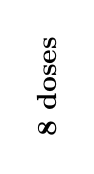
\begin{tikzpicture}
      \node[rotate=90] {\textbf{8 doses}};  
    \end{tikzpicture}
  \end{subfigure}  
  %
  \begin{subfigure}[c]{0.45\textwidth}
    
\includegraphics[width=\textwidth]{figures/dose-response-d_diff-1-2-3-8doses-dil8-bowl-neg-controls-0.055.png}
    %\caption{d diff 8doses-dil8-bowl-0.055}
    % \label{fig:tem}
  \end{subfigure} 
  %
  \begin{subfigure}[c]{0.45\textwidth}
    \centering
    
\includegraphics[width=\textwidth]{figures/dose-response-d_diff-1-2-3-8doses-dil8-bowl-neg-controls-0.085.png}
    %\caption{d diff 8doses-dil8-bowl-0.085}
    % \label{fig:tem}
  \end{subfigure}

  \begin{subfigure}[c]{0.05\textwidth}
    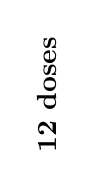
\begin{tikzpicture}
      \node[rotate=90] {\textbf{12 doses}};
    \end{tikzpicture}
  \end{subfigure}  
  % 
  \begin{subfigure}[c]{0.45\textwidth}
    
\includegraphics[width=\textwidth]{figures/dose-response-d_diff-1-2-3-12doses-dil4-bowl-neg-controls-0.055.png}
    %\caption{d diff 12doses-dil4-bowl-0.055}
    % \label{fig:tem}
  \end{subfigure} 
  %
  \begin{subfigure}[c]{0.45\textwidth}
    \centering
    
\includegraphics[width=\textwidth]{figures/dose-response-d_diff-1-2-3-12doses-dil4-bowl-neg-controls-0.085.png}
    %\caption{d diff 12doses-dil4-bowl-0.085}
    % \label{fig:tem}
  \end{subfigure}
  \caption{Mean absolute difference between expected and obtained
    heights (max value) for dose-response curves using various numbers
    of doses, replicates, and bowl-shaped plate-effect strengths. The
    4PL sigmoide curves were fitted using compound data and 4 negative
    controls such that their mean was equal to the mean of the 20
    negative controls the plate. *** indicates $p\leq10^{-43}$.}
\end{figure*}


%%% Local Variables: 
%%% mode: latex
%%% TeX-master: "supplement.tex"
%%% End: 
\input{tikz-figures/dose_response_d_dist_column_neg}

\input{tikz-figures/dose_response_relic50_bowl_no_neg}
\input{tikz-figures/dose_response_relic50_bowl_neg}
\begin{figure*}
  \centering
    \begin{subfigure}[c]{0.05\textwidth}
    ~
  \end{subfigure}
  % 
  \begin{subfigure}[c]{0.45\textwidth}
    \centering
    ~~\textbf{Mild plate effects}
  \end{subfigure}
  % 
  \begin{subfigure}[c]{0.45\textwidth}
    \centering
    ~~\textbf{Strong plate effects}
  \end{subfigure}

  \begin{subfigure}[c]{0.05\textwidth}
    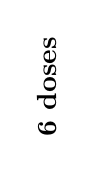
\begin{tikzpicture}
      \node[rotate=90] {\textbf{6 doses}};  
    \end{tikzpicture}
  \end{subfigure}  
  %
  \begin{subfigure}[c]{0.45\textwidth}
    
\includegraphics[width=\textwidth]{figures/dose-response-relic50-1-2-3-6doses-dil18-half-columns-neg-controls-0.2.png}
    %\caption{relic50 6doses-dil8-bowl-0.055}
    % \label{fig:tem}
  \end{subfigure}
  %
  \begin{subfigure}[c]{0.45\textwidth}
    \centering
    
\includegraphics[width=\textwidth]{figures/dose-response-relic50-1-2-3-6doses-dil18-half-columns-neg-controls-0.4.png}
    %\caption{relic50 6doses-dil18-bowl-0.085}
    % \label{fig:tem}
  \end{subfigure}

    \begin{subfigure}[c]{0.05\textwidth}
    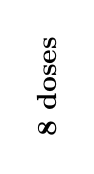
\begin{tikzpicture}
      \node[rotate=90] {\textbf{8 doses}};  
    \end{tikzpicture}
  \end{subfigure}  
  %
  \begin{subfigure}[c]{0.45\textwidth}
    
\includegraphics[width=\textwidth]{figures/dose-response-relic50-1-2-3-8doses-dil8-half-columns-neg-controls-0.2.png}
    %\caption{relic50 8doses-dil8-bowl-0.055}
    % \label{fig:tem}
  \end{subfigure} 
  %
  \begin{subfigure}[c]{0.45\textwidth}
    \centering
    
\includegraphics[width=\textwidth]{figures/dose-response-relic50-1-2-3-8doses-dil8-half-columns-neg-controls-0.4.png}
    %\caption{relic50 8doses-dil8-bowl-0.085}
    % \label{fig:tem}
  \end{subfigure}

    \begin{subfigure}[c]{0.05\textwidth}
    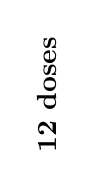
\begin{tikzpicture}
      \node[rotate=90] {\textbf{12 doses}};  
    \end{tikzpicture}
  \end{subfigure}  
  %
   \begin{subfigure}[c]{0.45\textwidth}
    
\includegraphics[width=\textwidth]{figures/dose-response-relic50-1-2-3-12doses-dil4-half-columns-neg-controls-0.2.png}
    %\caption{relic50 12doses-dil4-bowl-0.055}
    % \label{fig:tem}
  \end{subfigure} 
  %
  \begin{subfigure}[c]{0.45\textwidth}
    \centering
    
\includegraphics[width=\textwidth]{figures/dose-response-relic50-1-2-3-12doses-dil4-half-columns-neg-controls-0.4.png}
    %\caption{relic50 12doses-dil4-bowl-0.085}
    % \label{fig:tem}
  \end{subfigure}
  \caption{Mean absolute $\log_{10}$ difference between expected and
    obtained values of the relative
    {$\text{EC}_{50}$/$\text{IC}_{50}$} for dose-response curves using
    various numbers of doses, replicates, and plate-effect strengths
    with a linear relationship to column number in the right half of
    the plate. The 4PL sigmoide curves were fitted using compound data
    and 4 negative controls such that their mean was equal to the mean
    of the 20 negative controls the plate. * indicates $p\leq10^{-4}$,
    ** indicates $p\leq10^{-12}$, *** indicates $p\leq10^{-43}$.}
\end{figure*}



%%% Local Variables: 
%%% mode: latex
%%% TeX-master: "supplement.tex"
%%% End: 


\begin{figure*}
  \centering
  \begin{subfigure}[b]{0.05\textwidth}
    ~
  \end{subfigure}
  % 
  \begin{subfigure}[b]{0.45\textwidth}
    \centering
    ~~\textbf{Mild plate effects}
  \end{subfigure}
  % 
  \begin{subfigure}[b]{0.45\textwidth}
    \centering
    ~~\textbf{Strong plate effects}
  \end{subfigure}

  \begin{subfigure}[c]{0.05\textwidth}
    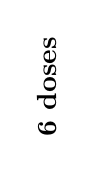
\begin{tikzpicture}
      \node[rotate=90] {\textbf{6 doses}};  
    \end{tikzpicture}
  \end{subfigure}  
  % 
  \begin{subfigure}[c]{0.45\textwidth}
    
\includegraphics[width=\textwidth]{figures/dose-response-absic50-1-2-3-6doses-dil18-bowl-0.055.png}
  \end{subfigure}
  %
  \begin{subfigure}[c]{0.45\textwidth}
    
\includegraphics[width=\textwidth]{figures/dose-response-absic50-1-2-3-6doses-dil18-bowl-0.085.png}
  \end{subfigure}

  \begin{subfigure}[c]{0.05\textwidth}
    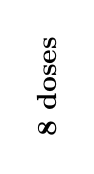
\begin{tikzpicture}
      \node[rotate=90] {\textbf{8 doses}};  
    \end{tikzpicture}
  \end{subfigure}  
  %
  \begin{subfigure}[c]{0.45\textwidth}
    
\includegraphics[width=\textwidth]{figures/dose-response-absic50-1-2-3-8doses-dil8-bowl-0.055.png} 
  \end{subfigure} 
  %
  \begin{subfigure}[c]{0.45\textwidth}
    
\includegraphics[width=\textwidth]{figures/dose-response-absic50-1-2-3-8doses-dil8-bowl-0.085.png}
  \end{subfigure}

  \begin{subfigure}[c]{0.05\textwidth}
    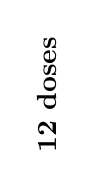
\begin{tikzpicture}
      \node[rotate=90] {\textbf{12 doses}};  
    \end{tikzpicture}
  \end{subfigure}  
  %
  \begin{subfigure}[c]{0.45\textwidth}
    \includegraphics[width=\textwidth]{figures/dose-response-absic50-1-2-3-12doses-dil4-bowl-0.055.png}
  \end{subfigure} 
  %
  \begin{subfigure}[c]{0.45\textwidth}
    \centering
     \includegraphics[width=\textwidth]{figures/dose-response-absic50-1-2-3-12doses-dil4-bowl-0.085.png}
  \end{subfigure}
  \caption{Mean absolute $\log_{10}$ difference between expected and
    obtained values of the absolute
    {$\text{EC}_{50}$/$\text{IC}_{50}$} for dose-response curves using
    various numbers of doses, replicates, and bowl-shaped plate-effect
    strengths. The 4PL sigmoide curves were fitted using only compound
    data. *** indicates $p<10^{-43}$.}
\end{figure*}


%%% Local Variables: 
%%% mode: latex
%%% TeX-master: "../supplement.tex"
%%% End: 
\begin{figure*}
  \centering
  \begin{subfigure}[b]{0.05\textwidth}
    ~
  \end{subfigure}
  % 
  \begin{subfigure}[b]{0.45\textwidth}
    \centering
    ~~\textbf{Mild plate effects}
  \end{subfigure}
  % 
  \begin{subfigure}[b]{0.45\textwidth}
    \centering
    ~~\textbf{Strong plate effects}
  \end{subfigure}

  \begin{subfigure}[c]{0.05\textwidth}
    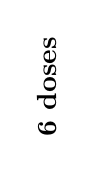
\begin{tikzpicture}
      \node[rotate=90] {\textbf{6 doses}};  
    \end{tikzpicture}
  \end{subfigure}  
  %
  \begin{subfigure}[c]{0.45\textwidth}
    
\includegraphics[width=\textwidth]{figures/dose-response-absic50-1-2-3-6doses-dil18-bowl-neg-controls-0.055.png}
%    \caption{}
    % \label{fig:tem}
  \end{subfigure}
  %
  \begin{subfigure}[c]{0.45\textwidth}
    \centering
    
\includegraphics[width=\textwidth]{figures/dose-response-absic50-1-2-3-6doses-dil18-bowl-neg-controls-0.085.png}
    %\caption{absic50 6doses-dil18-bowl-0.085} 
    % \label{fig:tem}
  \end{subfigure}

  \begin{subfigure}[c]{0.05\textwidth}
    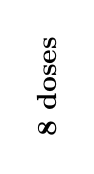
\begin{tikzpicture}
      \node[rotate=90] {\textbf{8 doses}};  
    \end{tikzpicture}
  \end{subfigure}  
  %
  \begin{subfigure}[c]{0.45\textwidth}
    
\includegraphics[width=\textwidth]{figures/dose-response-absic50-1-2-3-8doses-dil8-bowl-neg-controls-0.055.png}
    %\caption{absic50 8doses-dil8-bowl-0.055}
    % \label{fig:tem}
  \end{subfigure} 
  %
  \begin{subfigure}[c]{0.45\textwidth}
    \centering
    
\includegraphics[width=\textwidth]{figures/dose-response-absic50-1-2-3-8doses-dil8-bowl-neg-controls-0.085.png}
    % \caption{-}
    % \label{fig:} 
  \end{subfigure}
 
  \begin{subfigure}[c]{0.05\textwidth}
    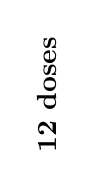
\begin{tikzpicture}
      \node[rotate=90] {\textbf{12 doses}};  
    \end{tikzpicture}
  \end{subfigure}  
  %
  \begin{subfigure}[c]{0.45\textwidth}
    \includegraphics[width=\textwidth]{figures/dose-response-absic50-1-2-3-12doses-dil4-bowl-neg-controls-0.055.png}
    %\caption{}
    % \label{fig:}
  \end{subfigure} 
  %
  \begin{subfigure}[c]{0.45\textwidth}
    \centering
    \includegraphics[width=\textwidth]{figures/dose-response-absic50-1-2-3-12doses-dil4-bowl-neg-controls-0.085.png}
    %\caption{absic50 12doses-dil4-bowl-0.085}
    % \label{fig:tem} 
  \end{subfigure}
  \caption{Mean absolute $\log_{10}$ difference between expected and
    obtained values of the absolute
    {$\text{EC}_{50}$/$\text{IC}_{50}$} for dose-response curves using
    various numbers of doses, replicates, and bowl-shaped plate-effect
    strengths. The 4PL sigmoide curves were fitted using compound data
    and 4 negative controls such that their mean was equal to the mean
    of the 20 negative controls the plate. *** indicates
    $p\leq10^{-43}$.}
\end{figure*}


%%% Local Variables: 
%%% mode: latex
%%% TeX-master: "supplement.tex"
%%% End:
\input{tikz-figures/dose_response_absic50_column_neg}

\input{tikz-figures/dose_response_residuals_bowl_no_neg}
\begin{figure*}
  \centering
    \begin{subfigure}[c]{0.05\textwidth}
    ~
  \end{subfigure}
  % 
  \begin{subfigure}[c]{0.45\textwidth}
    \centering
    ~~\textbf{Mild plate effects}
  \end{subfigure}
  % 
  \begin{subfigure}[c]{0.45\textwidth}
    \centering
    ~~\textbf{Strong plate effects}
  \end{subfigure}

  \begin{subfigure}[c]{0.05\textwidth}
    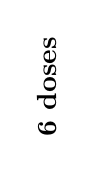
\begin{tikzpicture}
      \node[rotate=90] {\textbf{6 doses}};  
    \end{tikzpicture}
  \end{subfigure}  
  %
  \begin{subfigure}[c]{0.45\textwidth}
    
\includegraphics[width=\textwidth]{figures/residuals-1-2-3-6doses-dil18-half-columns-neg-controls-0.2.png}
    %\caption{Residuals 6doses-dil8-bowl-0.055}
    % \label{fig:tem}
  \end{subfigure}
  %
  \begin{subfigure}[c]{0.45\textwidth}
    \centering
    
\includegraphics[width=\textwidth]{figures/residuals-1-2-3-6doses-dil18-half-columns-neg-controls-0.4.png}
    %\caption{Residuals 6doses-dil18-bowl-0.085}
    % \label{fig:tem}
  \end{subfigure}

    \begin{subfigure}[c]{0.05\textwidth}
    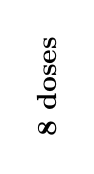
\begin{tikzpicture}
      \node[rotate=90] {\textbf{8 doses}};  
    \end{tikzpicture}
  \end{subfigure}  
  %
  \begin{subfigure}[c]{0.45\textwidth}
    
\includegraphics[width=\textwidth]{figures/residuals-1-2-3-8doses-dil8-half-columns-neg-controls-0.2.png}
    %\caption{Residuals 8doses-dil8-bowl-0.055}
    % \label{fig:tem}
  \end{subfigure} 
  %
  \begin{subfigure}[c]{0.45\textwidth}
    \centering
    
\includegraphics[width=\textwidth]{figures/residuals-1-2-3-8doses-dil8-half-columns-neg-controls-0.4.png}
    %\caption{Residuals 8doses-dil8-bowl-0.085}
    % \label{fig:tem}
  \end{subfigure}

    \begin{subfigure}[c]{0.05\textwidth}
    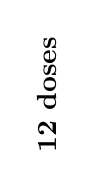
\begin{tikzpicture}
      \node[rotate=90] {\textbf{12 doses}};  
    \end{tikzpicture}
  \end{subfigure}  
  %
   \begin{subfigure}[c]{0.45\textwidth}
    
\includegraphics[width=\textwidth]{figures/residuals-1-2-3-12doses-dil4-half-columns-neg-controls-0.2.png}
    %\caption{Residuals 12doses-dil4-bowl-0.055}
    % \label{fig:tem}
  \end{subfigure} 
  %
  \begin{subfigure}[c]{0.45\textwidth}
    \centering
    
\includegraphics[width=\textwidth]{figures/residuals-1-2-3-12doses-dil4-half-columns-neg-controls-0.4.png}
    %\caption{Residuals 12doses-dil4-bowl-0.085}
    % \label{fig:tem}
  \end{subfigure}
  \caption{Residuals (MSE between expected and obtained responses) for
    dose-response simulations using various numbers of doses,
    replicates, and plate-effect strengths with a linear relationship
    to column number in the right half of the plate. *** indicates
    $p\leq10^{-43}$.}
    
\end{figure*}


%%% Local Variables: 
%%% mode: latex
%%% TeX-master: "supplement.tex"
%%% End: 

\begin{figure*}
  \centering
    \begin{subfigure}[c]{0.05\textwidth}
    ~
  \end{subfigure}
  % 
  \begin{subfigure}[c]{0.45\textwidth}
    \centering
    ~~\textbf{Mild plate effects}
  \end{subfigure}
  % 
  \begin{subfigure}[c]{0.45\textwidth}
    \centering
    ~~\textbf{Strong plate effects}
  \end{subfigure}

  \begin{subfigure}[c]{0.05\textwidth}
    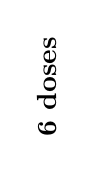
\begin{tikzpicture}
      \node[rotate=90] {\textbf{6 doses}};  
    \end{tikzpicture}
  \end{subfigure}  
  %
  \begin{subfigure}[c]{0.45\textwidth}
    
\includegraphics[width=\textwidth]{figures/percentage-low-r2-curves-1-2-3-6doses-dil18-bowl-0.055.png}
    %\caption{6doses-dil8-bowl-0.055}
    % \label{fig:tem}
  \end{subfigure}
  %
  \begin{subfigure}[c]{0.45\textwidth}
    \centering
    
\includegraphics[width=\textwidth]{figures/percentage-low-r2-curves-1-2-3-6doses-dil18-bowl-0.085.png}
    %\caption{6doses-dil18-bowl-0.085}
    % \label{fig:tem}
  \end{subfigure}

  \begin{subfigure}[c]{0.05\textwidth}
    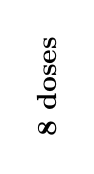
\begin{tikzpicture}
      \node[rotate=90] {\textbf{8 doses}};  
    \end{tikzpicture}
  \end{subfigure}  
  %
  \begin{subfigure}[c]{0.45\textwidth}
    
\includegraphics[width=\textwidth]{figures/percentage-low-r2-curves-1-2-3-8doses-dil8-bowl-0.055.png}
    %\caption{8doses-dil8-bowl-0.055}
    % \label{fig:tem}
  \end{subfigure} 
  %
  \begin{subfigure}[c]{0.45\textwidth}
    \centering
    
\includegraphics[width=\textwidth]{figures/percentage-low-r2-curves-1-2-3-8doses-dil8-bowl-0.085.png}
    %\caption{8doses-dil8-bowl-0.085}
    % \label{fig:tem}
  \end{subfigure}

  \begin{subfigure}[c]{0.05\textwidth}
    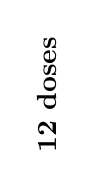
\begin{tikzpicture}
      \node[rotate=90] {\textbf{12 doses}};  
    \end{tikzpicture}
  \end{subfigure}  
  %
   \begin{subfigure}[c]{0.45\textwidth}
    
\includegraphics[width=\textwidth]{figures/percentage-low-r2-curves-1-2-3-12doses-dil4-bowl-0.055.png}
    %\caption{12doses-dil4-bowl-0.055}
    % \label{fig:tem}
  \end{subfigure} 
  %
  \begin{subfigure}[c]{0.45\textwidth}
    \centering
    
\includegraphics[width=\textwidth]{figures/percentage-low-r2-curves-1-2-3-12doses-dil4-bowl-0.085.png}
    %\caption{Residuals 12doses-dil4-bowl-0.085}
    % \label{fig:tem}
  \end{subfigure}
  \caption{Percentage of dose-response curves with low-quality
    ($R^2 < 80\%$) using various numbers of doses, replicates, and
    bowl-shaped plate-effect strengths. The 4PL sigmoide curves were
    fitted using only compound data.}
\end{figure*}



%%% Local Variables: 
%%% mode: latex
%%% TeX-master: "supplement.tex"
%%% End: 
\begin{figure*}
  \centering
    \begin{subfigure}[c]{0.05\textwidth}
    ~
  \end{subfigure}
  % 
  \begin{subfigure}[c]{0.45\textwidth}
    \centering
    ~~\textbf{Mild plate effects}
  \end{subfigure}
  % 
  \begin{subfigure}[c]{0.45\textwidth}
    \centering
    ~~\textbf{Strong plate effects}
  \end{subfigure}

  \begin{subfigure}[c]{0.05\textwidth}
    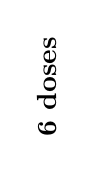
\begin{tikzpicture}
      \node[rotate=90] {\textbf{6 doses}};  
    \end{tikzpicture}
  \end{subfigure}  
  %
  \begin{subfigure}[c]{0.45\textwidth}
    
\includegraphics[width=\textwidth]{figures/percentage-low-r2-curves-1-2-3-6doses-dil18-bowl-neg-controls-0.055.png}
    %\caption{6doses-dil8-bowl-0.055}
    % \label{fig:tem}
  \end{subfigure}
  %
  \begin{subfigure}[c]{0.45\textwidth}
    \centering
    
\includegraphics[width=\textwidth]{figures/percentage-low-r2-curves-1-2-3-6doses-dil18-bowl-neg-controls-0.085.png}
    %\caption{6doses-dil18-bowl-0.085}
    % \label{fig:tem}
  \end{subfigure}

  \begin{subfigure}[c]{0.05\textwidth}
    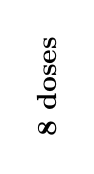
\begin{tikzpicture}
      \node[rotate=90] {\textbf{8 doses}};  
    \end{tikzpicture}
  \end{subfigure}  
  %
  \begin{subfigure}[c]{0.45\textwidth}
    
\includegraphics[width=\textwidth]{figures/percentage-low-r2-curves-1-2-3-8doses-dil8-bowl-neg-controls-0.055.png}
    %\caption{8doses-dil8-bowl-0.055}
    % \label{fig:tem}
  \end{subfigure} 
  %
  \begin{subfigure}[c]{0.45\textwidth}
    \centering
    
\includegraphics[width=\textwidth]{figures/percentage-low-r2-curves-1-2-3-8doses-dil8-bowl-neg-controls-0.085.png}
    %\caption{8doses-dil8-bowl-0.085}
    % \label{fig:tem}
  \end{subfigure}

  \begin{subfigure}[c]{0.05\textwidth}
    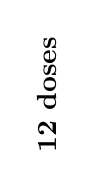
\begin{tikzpicture}
      \node[rotate=90] {\textbf{12 doses}};  
    \end{tikzpicture}
  \end{subfigure}  
  %
   \begin{subfigure}[c]{0.45\textwidth}
    
\includegraphics[width=\textwidth]{figures/percentage-low-r2-curves-1-2-3-12doses-dil4-bowl-neg-controls-0.055.png}
    %\caption{12doses-dil4-bowl-0.055}
    % \label{fig:tem}
  \end{subfigure} 
  %
  \begin{subfigure}[c]{0.45\textwidth}
    \centering
    
\includegraphics[width=\textwidth]{figures/percentage-low-r2-curves-1-2-3-12doses-dil4-bowl-neg-controls-0.085.png}
    %\caption{Residuals 12doses-dil4-bowl-0.085}
    % \label{fig:tem}
  \end{subfigure}
  \caption{Percentage of dose-response curves with low-quality
    ($R^2 < 80\%$) using various numbers of doses, replicates, and
    bowl-shaped plate-effect strengths. The 4PL sigmoide curves were
    fitted using compound data and 4 negative controls such that their
    mean was equal to the mean of the 20 negative controls the plate.}
\end{figure*}



%%% Local Variables: 
%%% mode: latex
%%% TeX-master: "supplement.tex"
%%% End: 
\input{tikz-figures/dose_response_percentage_column_neg}

\begin{figure*}
  \centering     
     %   \begin{subfigure}[b]{0.49\textwidth}
     %   \caption{Expected}
     %     
\includegraphics[width=\textwidth]{figures/screening-bowl-0.03-10-10-0.99-stdev-3-4-expected.png}
     %     \label{fig:expected}
     % \end{subfigure}
     % \hfill


       \begin{subfigure}[b]{0.31\textwidth}
         \centering
         \caption{Random}
         
\includegraphics[width=\textwidth]{figures/screening-bowl-0.03-10-10-0.99-stdev-3-4-random.png}
         %\label{fig:random}
     \end{subfigure}
     \hfill
     \begin{subfigure}[b]{0.31\textwidth}
         \centering
         \caption{PLAID}
         
\includegraphics[width=\textwidth]{figures/screening-bowl-0.03-10-10-0.99-stdev-3-4-plaid.png}
         %\label{fig:effective}
     \end{subfigure}
     \hfill
     \begin{subfigure}[b]{0.31\textwidth}
         \centering
         \caption{COMPD}
         
\includegraphics[width=\textwidth]{figures/screening-bowl-0.03-10-10-0.99-stdev-3-4-compd.png}
         %\label{fig:border}
     \end{subfigure}
  
     \caption{Comparison between expected and obtained values for
       screening experiments using $10$~positive and $10$~negative
       controls on 384-well plates with only 1~replicate, 1\%~hit-rate
       and mild bowl-shaped plate effects.} 
        \label{fig:screening-data-collection-mild}
\end{figure*}
\input{tikz-figures/screening_data_expected_obtained2}
\input{tikz-figures/screening_data_expected_obtained3}




\begin{figure*}
  \begin{subfigure}[b]{0.49\textwidth}
    \centering
    
\includegraphics[width=\textwidth]{figures/ROC-10-10-0.2-1.png}
    \caption{1\% hits}
    %\label{fig:plaid-control-layout-bowl}
  \end{subfigure}
  \hfill
  \begin{subfigure}[b]{0.49\textwidth}
    \centering
    
\includegraphics[width=\textwidth]{figures/ROC-10-10-0.2-5.png}
    \caption{5\% hits}
    %\label{fig:plaid-control-layout-bowl}
  \end{subfigure}

  
  \begin{subfigure}[b]{0.49\textwidth}
    \centering
    
\includegraphics[width=\textwidth]{figures/ROC-10-10-0.2-10.png}
    \caption{10\% hits}
    %\label{fig:plaid-control-layout-bowl}
  \end{subfigure}
  \hfill
  \begin{subfigure}[b]{0.49\textwidth}
    \centering
    
\includegraphics[width=\textwidth]{figures/ROC-10-10-0.2-20.png}
    \caption{20\% hits}
    %\label{fig:plaid-control-layout-bowl}
  \end{subfigure}

  \begin{subfigure}[b]{0.49\textwidth}
    \centering
    
\includegraphics[width=\textwidth]{figures/ROC-10-10-0.2-30.png}
    \caption{30\% hits}
    %\label{fig:plaid-control-layout-bowl}
  \end{subfigure}
  \hfill
  \begin{subfigure}[b]{0.49\textwidth}
    \centering
    
\includegraphics[width=\textwidth]{figures/ROC-10-10-0.2-40.png}
    \caption{40\% hits}
    %\label{fig:plaid-control-layout-bowl}
  \end{subfigure}
  
  \caption{Comparison of ROC curves for screening experiments with
    different hit rates, using layouts with 10 positive and 10
    negative controls in the presence of strong bowl-shaped plate
    effects.}
    \label{fig:screening-roc-10-10}
\end{figure*}




%%% Local Variables: 
%%% mode: latex
%%% TeX-master: "../supplement.tex"
%%% End: 

\input{tikz-figures/screening_data_roc_strong_8_8}

\input{tikz-figures/screening_data_pr_strong}



\begin{figure*}
    \begin{subfigure}[b]{0.49\textwidth}
    \centering
    
\includegraphics[width=\textwidth]{figures/PR-8-8-0.1-1.png}
    \caption{1\% hits}
    %\label{fig:plaid-control-layout-bowl}
  \end{subfigure}
  \hfill
  \begin{subfigure}[b]{0.49\textwidth}
    \centering
    
\includegraphics[width=\textwidth]{figures/PR-8-8-0.1-5.png}
    \caption{5\% hits}
    %\label{fig:plaid-control-layout-bowl}
  \end{subfigure}

  
  \begin{subfigure}[b]{0.49\textwidth}
    \centering
    
\includegraphics[width=\textwidth]{figures/PR-8-8-0.1-10.png}
    \caption{10\% hits}
    %\label{fig:plaid-control-layout-bowl}
  \end{subfigure}
  \hfill
  \begin{subfigure}[b]{0.49\textwidth}
    \centering
    
\includegraphics[width=\textwidth]{figures/PR-8-8-0.1-20.png}
    \caption{20\% hits}
    %\label{fig:plaid-control-layout-bowl}
  \end{subfigure}

  \begin{subfigure}[b]{0.49\textwidth}
    \centering
    
\includegraphics[width=\textwidth]{figures/PR-8-8-0.1-30.png}
    \caption{30\% hits}
    %\label{fig:plaid-control-layout-bowl}
  \end{subfigure}
  \hfill
  \begin{subfigure}[b]{0.49\textwidth}
    \centering
    
\includegraphics[width=\textwidth]{figures/PR-8-8-0.1-40.png}
    \caption{40\% hits}
    %\label{fig:plaid-control-layout-bowl}
  \end{subfigure}
  
  \caption{Comparison of PR curves for screening experiments with
    different hit rates, using layouts with 8 positive and 8
    negative controls in the presence of moderate bowl-shaped plate
    effects.}
    \label{fig:screening-pr-8-8}
\end{figure*}




%%% Local Variables: 
%%% mode: latex
%%% TeX-master: "../supplement.tex"
%%% End: 


\begin{figure*}
  \centering
  \begin{subfigure}[b]{0.3\textwidth}
    \centering
    \caption{No plate effect} 
\includegraphics[width=\textwidth]{figures/screening-Zfactor-mse-screening_metrics_data-10-10-0.0-20250623-reviewing.csv.png}
    \label{fig:zfactor_1}
  \end{subfigure}
  \hfill
  \begin{subfigure}[b]{0.3\textwidth}
    \centering
    \caption{1} 
\includegraphics[width=\textwidth]{figures/screening-Zfactor-mse-screening_metrics_data-10-10-0.01-20250623-reviewing.csv.png}
    \label{fig:zfactor_2}
  \end{subfigure}
    \hfill
  \begin{subfigure}[b]{0.3\textwidth}
    \caption{2} 
\includegraphics[width=\textwidth]{figures/screening-Zfactor-mse-screening_metrics_data-10-10-0.02-20250623-reviewing.csv.png}
    \label{fig:zfactor_3}
  \end{subfigure}



    \begin{subfigure}[b]{0.3\textwidth}
    \centering
    \caption{3} 
\includegraphics[width=\textwidth]{figures/screening-Zfactor-mse-screening_metrics_data-10-10-0.03-20250623-reviewing.csv.png}
    \label{fig:zfactor_4}
  \end{subfigure}
    \hfill
  \begin{subfigure}[b]{0.3\textwidth}
    \centering
    \caption{4} 
\includegraphics[width=\textwidth]{figures/screening-Zfactor-mse-screening_metrics_data-10-10-0.04-20250623-reviewing.csv.png}
    \label{fig:zfactor_5}
  \end{subfigure}
  \hfill
  \begin{subfigure}[b]{0.3\textwidth}
    \centering
    \caption{5} 
\includegraphics[width=\textwidth]{figures/screening-Zfactor-mse-screening_metrics_data-10-10-0.05-20250623-reviewing.csv.png}
    \label{fig:zfactor_6}
  \end{subfigure}


  
  
  \begin{subfigure}[b]{0.3\textwidth}
    \centering
    \caption{6} 
\includegraphics[width=\textwidth]{figures/screening-Zfactor-mse-screening_metrics_data-10-10-0.06-20250623-reviewing.csv.png}
    \label{fig:zfactor_7}
  \end{subfigure}
    \hfill
  \begin{subfigure}[b]{0.3\textwidth}
    \centering
    \caption{7} 
\includegraphics[width=\textwidth]{figures/screening-Zfactor-mse-screening_metrics_data-10-10-0.07-20250623-reviewing.csv.png}
    \label{fig:zfactor_8}
  \end{subfigure}
  \hfill
  \begin{subfigure}[b]{0.3\textwidth} 
    \centering
    \caption{8} 
\includegraphics[width=\textwidth]{figures/screening-Zfactor-mse-screening_metrics_data-10-10-0.08-20250623-reviewing.csv.png}
    \label{fig:zfactor_9}
  \end{subfigure}


  
  \caption{Comparison of MSE when calculating the SSMD of plates for
    screenings experiments using $10$~positive and $10$~negative
    controls on 384-well plate with only 1~replicate, 1\%~hit-rate and
    varying strengths of bowl-shaped plate effects. * indicates
    ${p<0.05}$, **~indicates ${p<10^{-2}}$, ***~indicates
    ${p<10^{-3}}$.}
  \label{fig:screening-zpscore-collection-10-10-stdev-3} 
\end{figure*}



%%% Local Variables: 
%%% mode: latex
%%% TeX-master: "supplement.tex"
%%% End: 



\input{tikz-figures/screening_data_ssmd}


\input{b_table_stats}

\bibliographystyle{plain}
\bibliography{compd_bibliography}


\end{document}